\chapter{Bitshield}
\label{chap:arc}
This chapter presents NAME, a set of changes to the dissemination algorithm of transactions with the objective of making it more efficient, namely by lowering the number of redundant advertisements that each node receives.
Section~\ref{sec:sm} presents the system model assumed by NAME, Section~\ref{sec:ranking} describes the process used by NAME to rank the different neighbours of a node, Section~\ref{sec:sr} details the algorithm used to take advantage of the ranking of neighbours and finally Section~\ref{sec:nc} presents the algorithm used by NAME to adapt to changes in the network.


\section{System model}
\label{sec:sm}

The system model that we considered when developing our solution was a system where nodes picked a random set of 8 nodes from the pool of nodes, and then establish a connection with those nodes. Nodes can not have more than 125 connections. When a node tries to establish a connection with another node, the other node will always accept it.

Regarding byzantine and rational nodes we only considered nodes that would not relay transactions as that was the only behaviour we found more profitable for a byzantine or rational miner.

In terms of architecture, the only module that would need to be tweaked is the broadcast module inside the Blockchain module as it is depicted in Figure~\ref{fig:arch}. Because as previously said this module is the one responsible for broadcasting the transactions and the blocks to the neighbours of a node.

\begin{figure}[h]
\centering
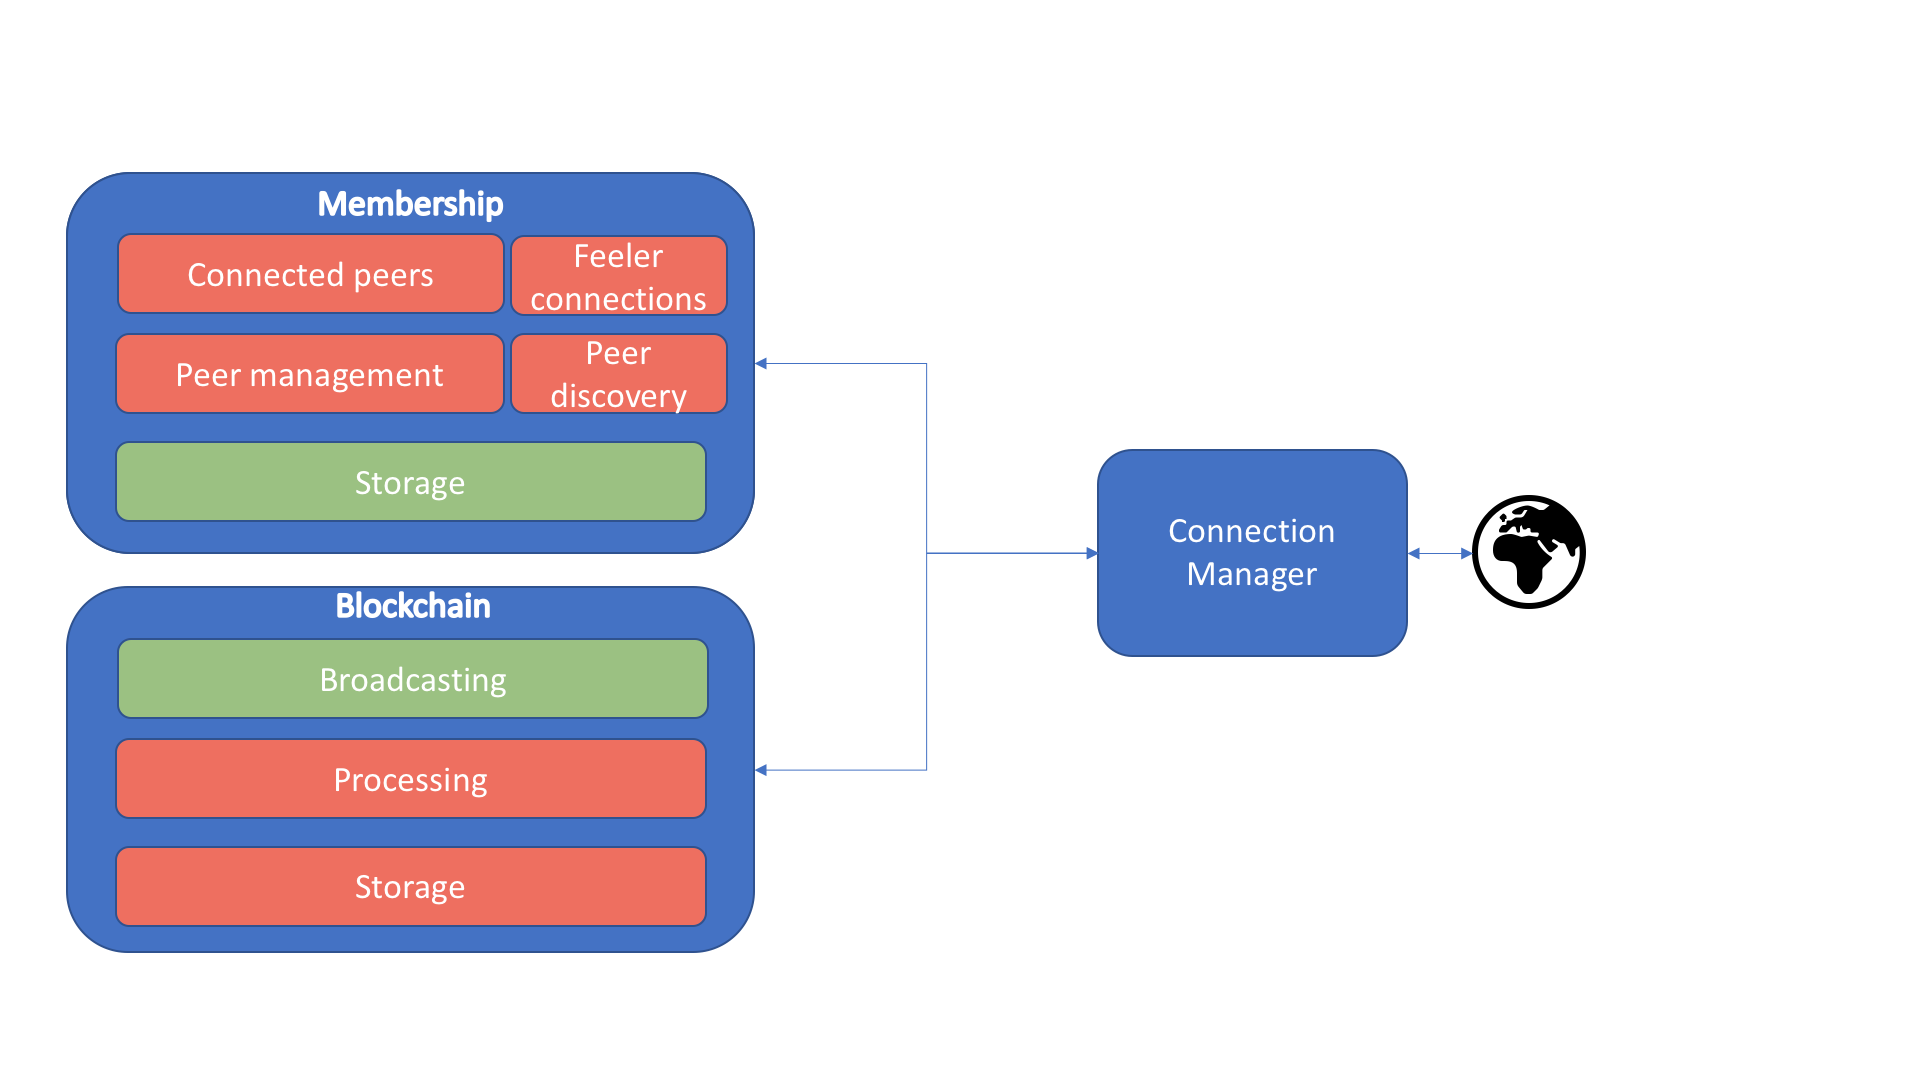
\includegraphics[scale=0.4]{figs/Architecture.png}
\caption{New Bitcoin architecture}
\label{fig:arch}
\end{figure}

We will now take a look at the ranking process.

\section{Ranking Neighbours}
\label{sec:ranking}
Our main objective is to lower the amount of duplicated advertisements in the network while ensuring that the transactions reach the miners. The intuition for the proposed approach is to skew the process of dissemination towards the most productive miners. However, this could put the resilience of the system at stake. To prevent this, we also broadcast transactions to the rest of the system through alternative paths.

Our approach encompasses three changes to the protocol.
First, nodes  maintain, for each neighbour, a list of the transactions sent by that neighbour and how long it took for these transactions to be included in a block.
Second, we also maintain for each neighbour the time, it took to send a block to the node.
Finally, nodes use these metrics to rank their neighbours and prioritise the dissemination of transaction accordingly.

To lower bandwidth usage, nodes prioritise neighbours that are closer to miners, or are miners themselves.
This is done in a decentralised fashion but results in fast paths to miners emerging over other paths.
Locally, each node, classifies neighbours as follows:

\begin{displaymath} \mbox{class}^{T}= (\dfrac{k^{T}}{n^{T}} + a^{T} - n^{T} + \dfrac{y^{T}}{z^{T}}) \end{displaymath}

%To solve the problem referenced in Section~\ref{} NAME takes advantage of asymmetries that already exists in the network. Namely the fact that the majority of blocks are mainly mined by mining pools with only a total of 11 (7.6\%) blocks mined in a day coming from unknown sources at the time of writing.

%With this information, the objective of NAME is to prioritize miners in the process of dissemination. To be able to do this the nodes have to discover the best path to the closest miners. Here the best path is the path that takes less time for the transactions of a node to reach a miner. We achieve this by ordering our neighbours by proximity to miners. Hence, the neighbours closest to miners will be on top of our ordering and the ones further away will be at the bottom.

where:
\begin{itemize}
  \item \textit{k} it the accumulated time it took to a neighbour to disseminate each block to the node;
  \item \textit{n} is the total number of blocks received by a neighbour;
  \item \textit{a} is the total number of blocks received;
  \item \textit{y} is the accumulated time it took for transactions, sent to a neighbour, to be accepted in a block;
  \item \textit{z} is the total number of transactions sent to a neighbour.
\end{itemize}

The time it takes for a neighbour to relay a block to a node is given by the difference between the current time and the last time the node received a new block from that neighbour.
%If a neighbour takes more than four hours to relay a block to a node, the difference will be the current time minus four hours.
This is to allow the classification to automatically adapt to situations where nodes that generate a block sparingly do not get a good classification indefinitely.
In fact, even though the majority of blocks is generated by a small subset of miners, sometimes a random node is able to mine a new block successfully.

Given the large number of transactions that flow through the network, instead of maintaining timers for all of them, we only maintain a timer every one hundred transactions. This prevents overloading nodes with metadata while still giving a good sample of the general network behaviour.

With his in mind, a neighbour has a good classification if it has a good ratio of \textsl{time it takes to disseminate blocks/number of blocks we received from him}, a good ratio of \textsl{blocks received from him/blocks received} and finally a good ratio of \textsl{time it took for a transaction to be added to blocks if we sent it to him}.

Given that the classification of neighbours is prone to change over time, the actual value used to order neighbours is given by the following sliding average of the classification presented previously:

\begin{displaymath} \mbox{class}^t = (1-\alpha) \cdot \mbox{class}^{t-1} + \alpha \cdot \mbox{class}^{T} \end{displaymath}

The $\alpha$ factor exists to avoid nodes that generated a lot of blocks in the past but no longer do, from having a good classification forever. In our experiments, we used an $\alpha=0.3$ and a \textit{T} configured to be an interval of four hours.

Each time a node receives a block from a neighbour the classification of the neighbours will be updated using Algorithm~\ref{alg:class}.

\begin{algorithm}[t]
\begin{algorithmic}[1]
\Function{update\_nodes\_classification}{node\_to\_update}
\State $scores \gets \textsl{[ ]}$
\For{$node$ \textbf{in} $neighbourhood$}
  \State $score \gets get\_classification(node)$
  \State $scores.append([score, id])$
\EndFor
\State $sort(scores)$
\State $top\_nodes \gets \textsl{[ ]}$
\For{$i$ \textbf{in} $range(0, max\_top\_nodes)$}
  \State $top\_nodes.append(score[i][1])$
\EndFor
\EndFunction
\end{algorithmic}
\caption{Top neighbours computation}
\label{alg:class}
\end{algorithm}

\section{Skewed relay}
\label{sec:sr}
%Given that our objective is that transactions reach a miner as fast as possible, we can use the mechanism described previously to do it.

If all nodes followed the protocol, it would suffice to use the mechanism described above to send
%Hence, if all the nodes were to follow the protocol correctly, and the paths created by out solution were resilient enough we could send our
transactions to only one node, as they would eventually appear in a block.

However, even if we do not consider the problem of node failure and Byzantine behaviour, there is the problem of commit time.
Briefly, the variance of the mining process could result in a prolific miner not being able to successfully mine a block for an extended period of time, precluding transactions sent exclusively to it from being included in the blockchain.
We address this - and simultaneously node failures and Byzantine behavior - by sending transactions not only to the \textsl{t} top nodes but also to \textsl{r} random nodes, as described in Algorithm~\ref{alg:diss}. This way we ensure that our transactions are still broadcast through the rest of the network and will be committed in a timely manner.

\begin{algorithm}[t]
\begin{algorithmic}[1]
\Function{nodes\_to\_send}{tx}
\If{$(ip == True$ \textbf{and} $tx.source() == self)$}
	\State {$\textbf{return}$ $neighbours$}
\EndIf
\State $total \gets max\_t\_nodes + max\_r\_nodes$
\If{$size(neighbours) < total$}
	\State $total \gets size(neighbours) - max\_t\_nodes$
\Else
	\State $total \gets total - max\_t\_nodes$
    \EndIf
\If{$total > 0$}
	\State $r\_nodes \gets rand\_choice(neighbours, max\_r\_nodes)$
    \EndIf
\State \Return t\_nodes + r\_nodes
\EndFunction
\end{algorithmic}
\caption{Nodes to send transactions advertisements computation}
\label{alg:diss}
\end{algorithm}

The variable \textsl{ip} (Initial Push) indicates that if a transaction is generated by a node, the node has the option of either sending it for only \textit{t} plus \textit{r} or to all his neighbours.

The dissemination process can then be configured with the following variables: \textsl{max\_top\_nodes}, \textsl{max\_random\_nodes} and \textsl{ip} to obtain different results in the information dissemination.
We study the impact of these parameters in Section~\ref{chap:evaluation}.

\section{Adapting to Network Changes}
\label{sec:nc}
A key aspect of peer-to-peer networks is that nodes can leave or join the network at any  time. With this in mind, we designed an algorithm that adapts to the network in order to maintain the commit time of the transactions while still trying to send as few messages as possible. As  depicted in Algorithm~\ref{alg:inc}, we automatically adjust the values of \textsl{max\_t\_nodes} and \textsl{max\_r\_nodes} depending on whether the node's transactions are taking too long to be committed or are being committed in a  timely fashion.

\begin{algorithm}[t]
\begin{algorithmic}[1]
\Function{increase\_relay}{}
\State $avg\_time \gets get\_avg\_time\_unconfirmed()$
\State $timeout \gets avg\_time() > TIME\_TX\_CONFIRM$
\State $space \gets max\_t\_nodes + 1 \leq neighbourhood / 2$
\State $cooldown \gets last\_inc + TIME\_TO\_WAIT \leq now$
\If{$timeout$ \textbf{and} $space$ \textbf{and} $cooldown$}
  \State $increase(t, r, 1)$
  \State $had\_to\_inc \gets True$
  \State $update\_nodes\_classification()$
  \State $last\_inc = now$
  \State $relay\_delayed\_TX()$
\EndIf
\State $cooldown \gets last\_dec + TIME\_TO\_WAIT \leq now$
\If{\textbf{not} $had\_to\_inc$ \textbf{and} $cooldown$}
  \State $avg\_time \gets get\_avg\_time\_confirmed()$
  \State $timeout \gets avg\_time() <= TIME\_TX\_CONFIRM$
  \State $space \gets max\_t\_nodes - 1 \leq 0$
  \If{$timeout$ \textbf{and} $space$}
    \State $decrease(t, r, 1)$
    \State $update\_nodes\_classification()$
    \State $last\_dec = now$
  \EndIf
\EndIf
\EndFunction
\end{algorithmic}
\caption{Increase or decrease top and random lists computation}
\label{alg:inc}
\end{algorithm}

Briefly, if the current average of the time it takes for the unconfirmed transactions of a node to be committed to a block, gets bigger than the constant \textsl{TIME\_TX\_CONFIRM} (30 minutes) then the node is going to increase both the size of \textsl{max\_t\_nodes} and \textsl{max\_r\_nodes}, and relay the transactions that took more than 30 minutes to commit.
If the average of all unconfirmed transactions does not surpass the threshold of the 30 minutes, the node will check if the average time it took to commit its confirmed transactions in the last hour took less than \textsl{TIME\_TX\_CONFIRM}. If so the node will lower the size of \textsl{max\_t\_nodes} and \textsl{max\_r\_nodes} by one, otherwise it will not do anything. Each time \textsl{max\_t\_nodes} and \textsl{max\_r\_nodes} are changed the node will not be able to change these values in the next 2 hours to prevent fluctuations in these values. Furthermore, every time a node increases \textsl{max\_t\_nodes} and \textsl{max\_r\_nodes} it will not be able to decrease these values in the next 4 hours in order to prioritise resilience over performance.

\section{Implementation}
\textbf{Have to write smth about this}
